% \AtBeginSection[]{
%     \begin{frame}
%         \frametitle{}
%         \tableofcontents[currentsection]
%     \end{frame}
% }

%%%%%%%%%%%%%%%%%%%%%%%%%%%%%%%%%%%%

\addtocounter{framenumber}{-1}

\section{Introduction}
\begin{frame}{Introduction}{Problem context}

    \begin{figure}
        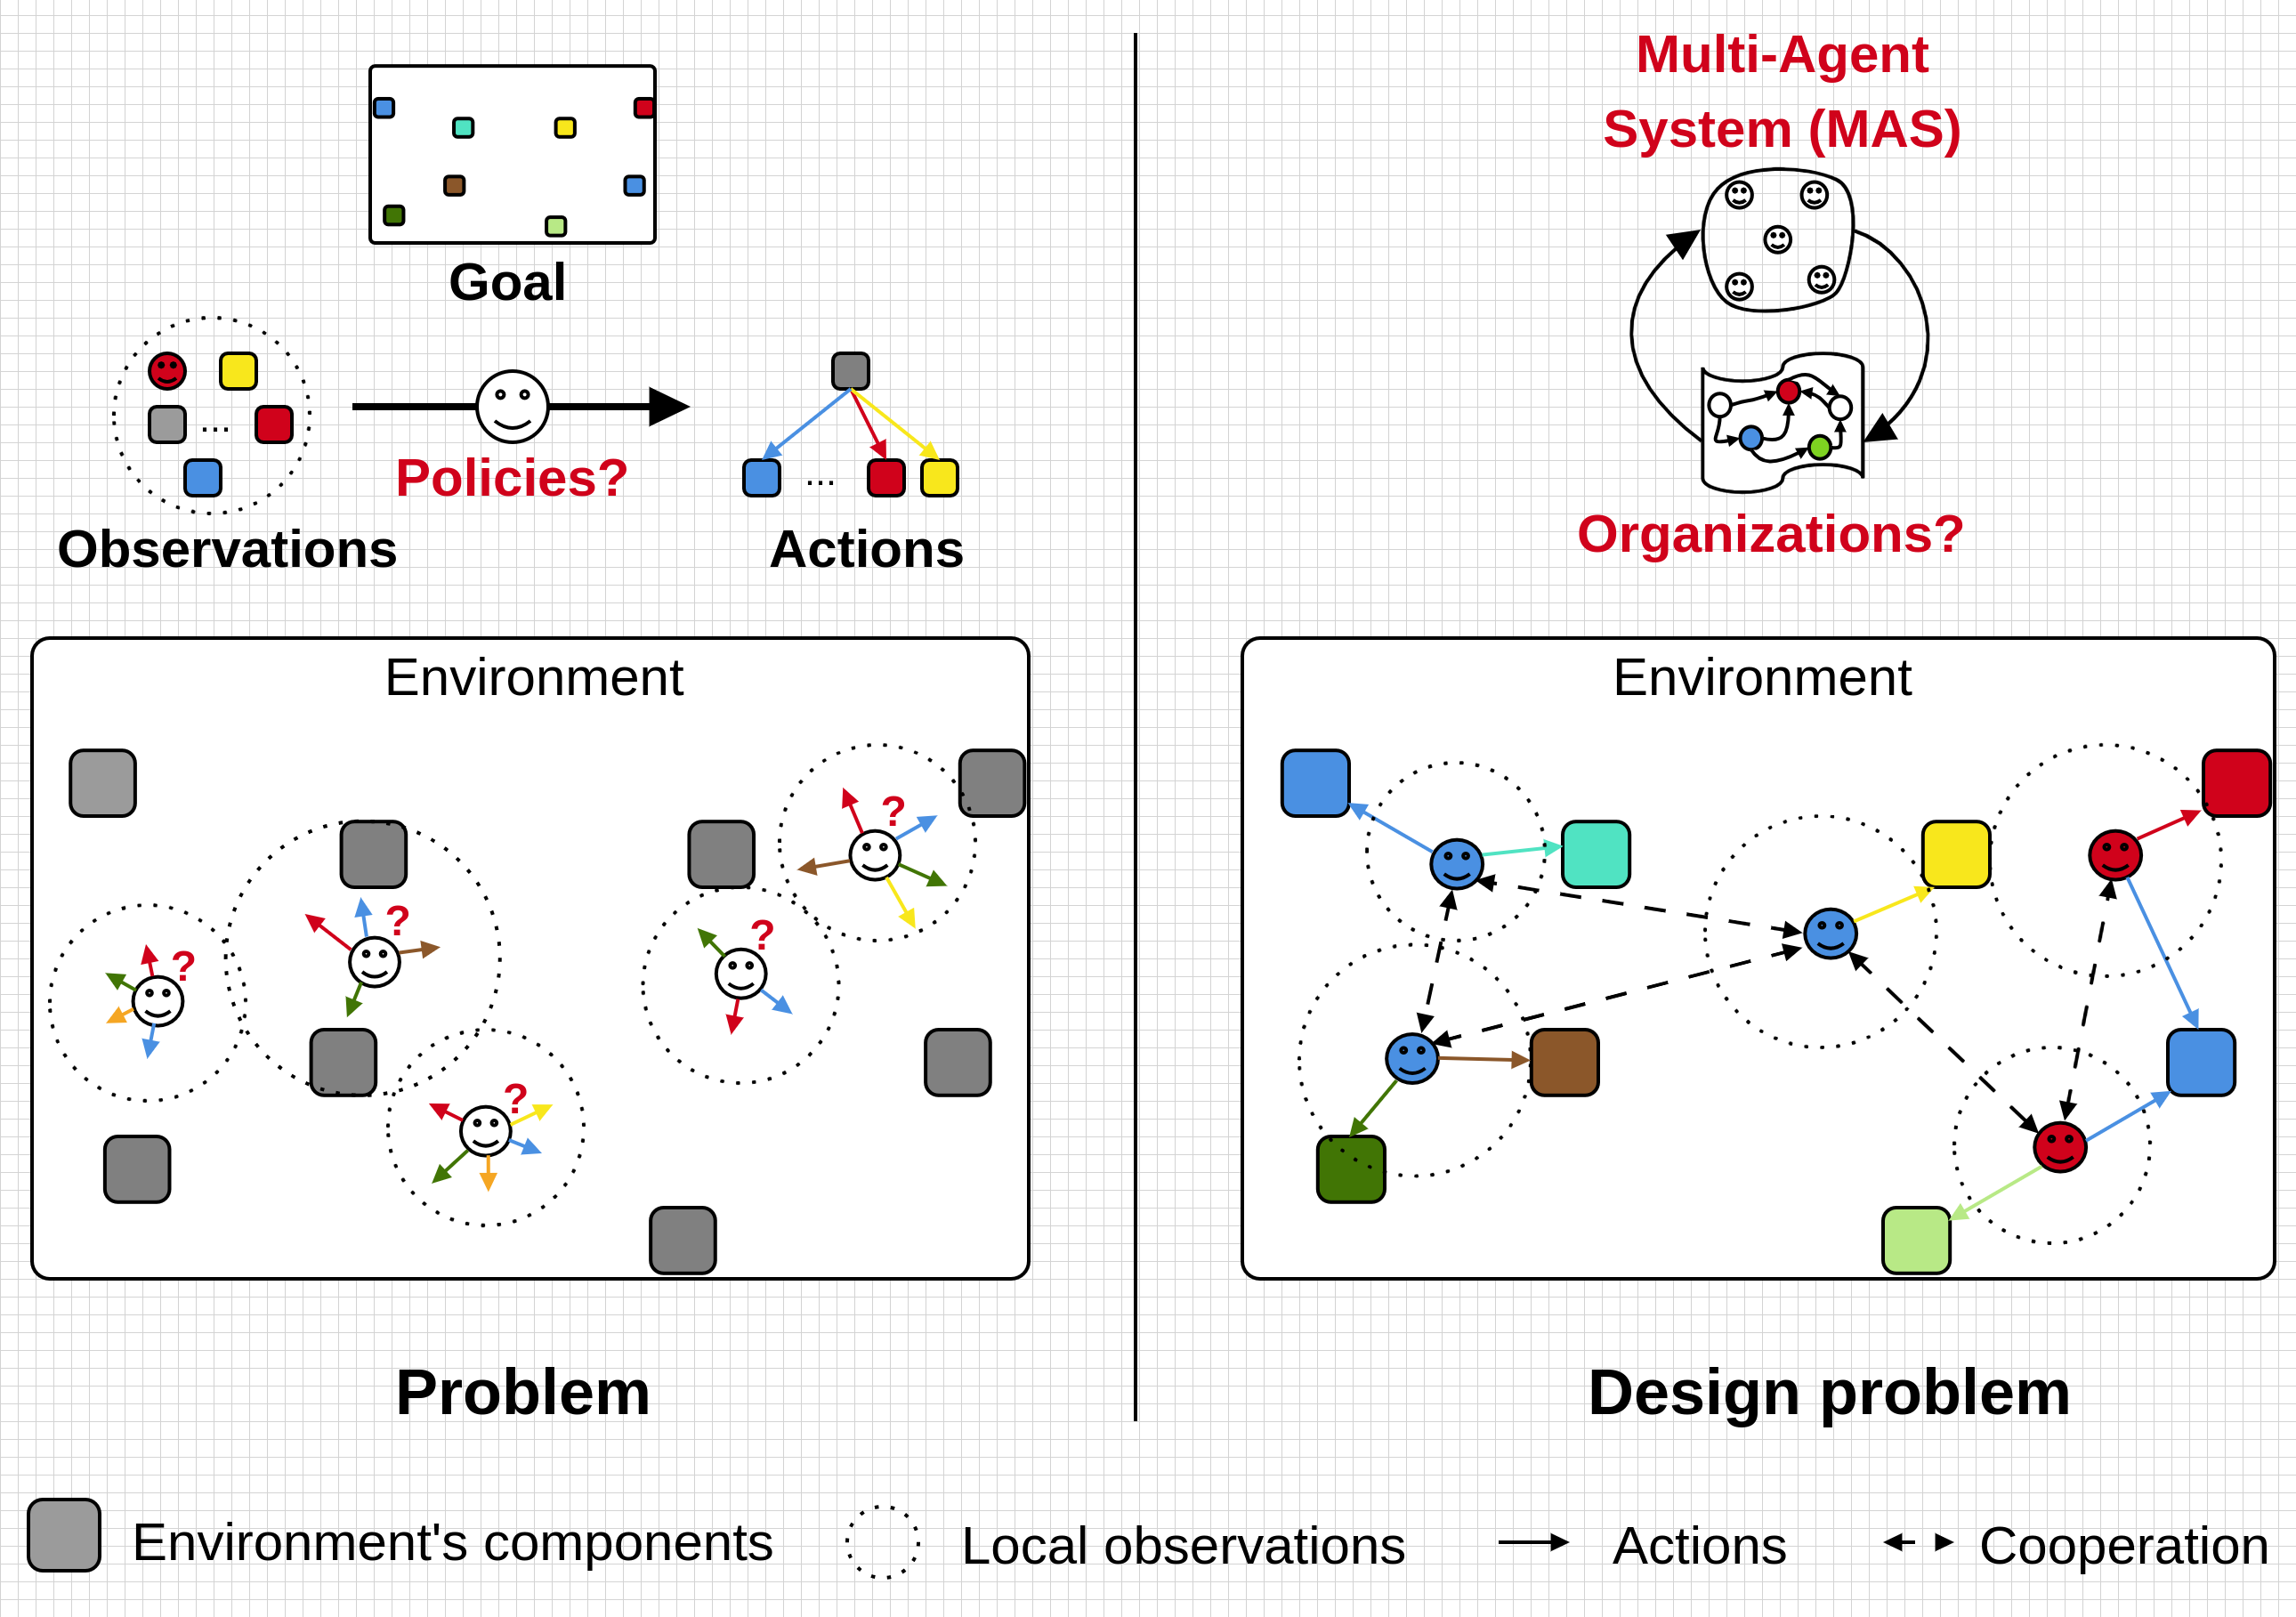
\includegraphics[width=0.9\linewidth]{figures/problem_illustration.png}
    \end{figure}

\end{frame}

\begin{frame}{Introduction}{Problem}


    \begin{alertblock}{Current design limitations}

        Methods require designers' experience but\dots

        \begin{itemize}
            \item \textbf{environment limitations}: complexity, limited access, non \dots
            \item \textbf{designers limitations}: availability, time consuming\dots
        \end{itemize}
        \vspace{1ex}
        $\Longrightarrow$ Increasing design knowledge $\rightarrow$ \textbf{costly}
    \end{alertblock}

    \begin{exampleblock}{\textbf{Example}: Autonomous Intelligent Cyberdefense Agents~\cite{Kott2023} (AICA)}

        \begin{columns}
            \hspace{5ex}
            \begin{column}{0.85\textwidth}
                \textbf{Cyberdefense Multi-Agent System}: malware identification, countermeasures\dots \\ \phantom{x} \\
                $\Longrightarrow$ No visual/intuitive comprehension of complex networked environments
            \end{column}
            \begin{column}{0.22\textwidth}
                \hspace{-2.5ex}
                
\includegraphics[width=0.8\linewidth]{figures/AICA_IWG.jpg}
            \end{column}
        \end{columns}

    \end{exampleblock}

    \begin{alertblock}{Targeted gaps}
        \begin{enumerate}
            \item Automating the search for suited agents' policies satisfying design constraints;
            \item Explicating the emerging organizational mechanisms to assist the hand-craft design.
        \end{enumerate}
    \end{alertblock}

\end{frame}
\begin{frame}{Introduction}{Addressing the gaps}

    \begin{prosblock}{Contribution: AOMEA}

        \textbf{Assisted MAS Organization Engineering Approach (AOMEA)} based upon:
        \begin{itemize}
            \item \textbf{Multi-Agent Reinforcement Learning (MARL)}: automatically find suitable joint-policies;
            \item \textbf{Organizational model (OM)}: formalize an implicit organization as \textbf{Organizational Specifications (OS)};
            \item \textbf{Link MARL \& OM}: link explicit OS with \textbf{histories}/\textbf{trajectories} of on-training policies.
        \end{itemize}

        \

        In order to:
        \begin{enumerate}
            \item \textbf{Constrain MARL}: design constraints to satisfy during training to achieve the goals;
            \item \textbf{Generate Organizational specifications}: automatically compute OS from agents' behaviors.

                  $\rightarrow$ exploitable insights into relevant mechanisms for MAS design.
        \end{enumerate}

    \end{prosblock}


\end{frame}